%%%%%%%%%%%%%%%%%%%%%%%%%%%%%%%%%%%%%%%%%%%%%%%%%%%%%%%%%%%%%%%%%%%%%%
\section{Contrib Module Installation}\label{sec:Contrib-Install}
%%%%%%%%%%%%%%%%%%%%%%%%%%%%%%%%%%%%%%%%%%%%%%%%%%%%%%%%%%%%%%%%%%%%%%

This section describes how to install various \Term{contrib modules}
in the Condor system.
Some of these modules are separate, optional pieces, not included in
the main distribution of Condor.
Others are integral parts of Condor taken from the development series
that have certain features users might want to install.
Examples are the new SMP-aware \Condor{startd} and the CondorView
collector.  
Both of these modules come with Condor version 6.1 and
later versions.
However, 
these separate modules may be installed,
maintaining most of the stable release,
while not
switching over to using the
development binaries.

%%%%%%%%%%%%%%%%%%%%%%%%%%%%%%%%%%%%%%%%%%%%%%%%%%%%%%%%%%%%%%%%%%%%%%
\subsection{\label{sec:CondorView-Client-Install}
Installing the CondorView Client Contrib Module} 
%%%%%%%%%%%%%%%%%%%%%%%%%%%%%%%%%%%%%%%%%%%%%%%%%%%%%%%%%%%%%%%%%%%%%%

% We refer to the make_stats program often in this section; make a
% macro for it.
\newcommand{\MakeStats}{\Prog{make\_stats}}

The CondorView Client Contrib module is used to automatically generate
World Wide Web pages to display usage statistics of a Condor
pool.
Included in the module is a shell script which invokes the \Condor{stats}
command to retrieve pool usage statistics from the CondorView server and
generate HTML pages from the results.  
Also included is a Java applet which graphically visualizes Condor 
usage information.  
Users can interact with the applet to customize the visualization and to
zoom in to a specific time frame.
Figure~\ref{fig:view-screenshot} on page~\pageref{fig:view-screenshot}
is a screen shot of a web page created by CondorView.  
To get a further feel for what pages generated by CondorView look like,
view the statistics for the University of Wisconsin-Madison pool
by visiting the URL \Url{http://www.cs.wisc.edu/condor} and clicking on
Condor View.

\begin{figure}[hbt]
\centering
\includegraphics{admin-man/view-screenshot.ps}
\caption{\label{fig:view-screenshot}Screenshot of CondorView Client}
\end{figure}

After unpacking and installing the CondorView Client, a script named
\MakeStats\ can be invoked to create HTML pages displaying Condor usage
for the past hour, day, week, or month.  
By using the Unix \Prog{cron} facility to periodically execute
\MakeStats, Condor pool usage statistics can be kept up to date
automatically.  
This simple model allows the CondorView Client to be easily installed;
no Web server CGI interface is needed.

%%%%%%%%%%%%%%%%%%%%%%%%%%%%%%%%%%%%%%%%%%%%%%%%%%%%%%%%%%%%%%%%%%%%%%
\subsubsection{\label{sec:condorview-client-step-by-step}
Step-by-Step Installation of the CondorView Client}
%%%%%%%%%%%%%%%%%%%%%%%%%%%%%%%%%%%%%%%%%%%%%%%%%%%%%%%%%%%%%%%%%%%%%%

\index{installation!CondorView Client}
\index{CondorView Client!installation}
\begin{enumerate}

\item Make certain that the CondorView Server is configured.
Section ~\ref{sec:Contrib-CondorView-Install}
describes configuration of the server.
The server logs information on disk in order to provide a persistent,
historical database of pool statistics.
The CondorView Client makes queries over the network to this
database.  The \Condor{collector} included with version 6.2.x and 6.1.x
Condor includes this database support.
To activate the persistent database logging, add the following entries to
the configuration file on the central manager: 
\begin{verbatim}
    POOL_HISTORY_DIR = /full/path/to/directory/to/store/historical/data 
    KEEP_POOL_HISTORY = True 
\end{verbatim}
For full details on these and other \condor{collector} configuration file
entries, see section~\ref{sec:Collector-Config-File-Entries} on
page~\pageref{sec:Collector-Config-File-Entries}.

\item Create a directory where CondorView is to place the HTML files.  
This directory should be one published by a web server, so that HTML
files which exist in this directory can be accessed using a web browser.  
This directory is referred to as the \File{VIEWDIR} directory.

\item Unpack or untar the CondorView Client Contrib module into the
directory \File{VIEWDIR}.
This creates several files and subdirectories.

\item Edit the \MakeStats script.  At the beginning of the file
are six parameters to customize.
The parameters are

        \begin{description}

	\item[\Macro{ORGNAME}] A brief name that identifies an
	organization. An example is ``Univ of Wisconsin''.  Do not
	use any slashes in the name or other special regular-expression
	characters. Avoid characters \Bs \^\ \$.

	\item[\Macro{CONDORADMIN}] The e-mail
	address of the Condor administrator at your site.  
	This e-mail address will appear at the bottom of the web pages.

	\item[\Macro{VIEWDIR}] The full pathname
	(\emph{not} a relative path) to the \File{VIEWDIR} directory set
	by installation step 2.  
	It is the directory that contains the \MakeStats\ script.

	\item[\Macro{STATSDIR}]  The full pathname of the
	directory which contains the \Condor{stats} binary.
	The \Condor{stats} program is included in the \Release{bin}
	directory with Condor version 6.1 and above; for Condor version
	6.0x, the \Condor{stats} program can be found in the CondorView
	Server Contrib module.
	The value for \Macro{STATSDIR} is added to the \Macro{PATH}
	parameter by default; see below.  

	\item[\Macro{PATH}] A list of subdirectories,
	separated by colons, where the \MakeStats\ script can find
	the \Prog{awk}, \Prog{bc}, \Prog{sed}, \Prog{date}, and \Condor{stats}
	programs.  
	If \Prog{perl} is installed, the path should also
	include the directory where \Prog{perl} is installed.
	The following default works on most systems:
        \begin{verbatim} 
        PATH=/bin:/usr/bin:$STATSDIR:/usr/local/bin
        \end{verbatim}

        \end{description}

\item To create all of the initial HTML files, type
\begin{verbatim}
        ./make_stats setup  
\end{verbatim}
Open the file \File{index.html} to verify that things look good.

\index{Condor\_View!use of\Prog{crontab} program}
\index{crontab program}

\item Add the \MakeStats\ program to \Prog{cron}.  
Running \MakeStats\ in step 5 created a \File{cronentries} file.
This \File{cronentries} file is ready to be processed by the Unix
\Prog{crontab} command.
The \Prog{crontab} manual page contains details about
the \Prog{crontab} command and the \Prog{cron} daemon.
Look at the
\File{cronentries} file; by default, it will run 
\Prog{\MakeStats\ hour} every 15 minutes, 
\Prog{\MakeStats\ day} once an hour, 
\Prog{\MakeStats\ week} twice per day, and 
\Prog{\MakeStats\ month} once per day.
These are reasonable defaults.  
You can add these commands to cron on any
system that can access the \MacroU{VIEWDIR} and
\MacroU{STATSDIR} directories,
even on a system that does not have Condor installed.
The commands do not need to run as user root; in
fact, they should probably not run as root.  These commands can run
as any user that has read/write access to the \File{VIEWDIR}.
To add these
commands to cron, enter : 
\begin{verbatim} 
        crontab cronentries
\end{verbatim}

\item Point the web browser at the \File{VIEWDIR} directory,
and to complete the installation.

\end{enumerate}

\index{CondorView!installation|)}

%%%%%%%%%%%%%%%%%%%%%%%%%%%%%%%%%%%%%%%%%%%%%%%%%%%%%%%%%%%%%%%%%%%%%%
\section{\label{sec:Ckpt-Server} The Checkpoint Server}
%%%%%%%%%%%%%%%%%%%%%%%%%%%%%%%%%%%%%%%%%%%%%%%%%%%%%%%%%%%%%%%%%%%%%%

\index{installation!checkpoint server}
\index{checkpoint server!installation|(}
A Checkpoint Server maintains a repository for checkpoint files.
Using checkpoint servers reduces the disk requirements of submitting
machines in the pool, since the submitting machines no longer need to
store checkpoint files locally.
Checkpoint server machines should have a large amount of disk space
available, and they should have a fast connection to machines
in the Condor pool.

If your spool directories are on a network file system, then
checkpoint files will make two trips over the network: one between the
submitting machine and the execution machine, and a second between the
submitting machine and the network file server.
If you install a checkpoint server and configure it to use the
server's local disk, the checkpoint will travel only once over the
network, between the execution machine and the checkpoint server.
You may also obtain checkpointing network performance benefits by
using multiple checkpoint servers, as discussed below.

\Note It is a good idea to pick very stable machines for your checkpoint
servers.
If individual checkpoint servers crash, the Condor system will continue to
operate, although poorly.  
While the Condor system will recover from a checkpoint server crash
as best it can, there are two problems that can (and will) occur:
\begin{enumerate}

\item A checkpoint cannot be sent to a checkpoint server that
is not functioning.
Jobs will keep trying to contact the checkpoint server, backing
off exponentially in the time they wait between attempts.
Normally, jobs only have a limited time to checkpoint before they are
kicked off the machine.
So, if the server is down for a long period of time, chances are that
a lot of work will be lost by jobs being killed without writing a
checkpoint. 

\item If a checkpoint is not available from the checkpoint
server, a job cannot be
retrieved, and it will either have to be restarted from
the beginning, or the job will wait for the server to come back online.
This behavior is controlled with the
\Macro{MAX\_DISCARDED\_RUN\_TIME} parameter in the config file (see
section~\ref{Checkpoint-Server-Config-File-Entries} on
page~\pageref{Checkpoint-Server-Config-File-Entries} for details).
This parameter represents the maximum amount of CPU time you are
willing to discard by starting a job over from scratch if the
checkpoint server is not responding to requests.

\end{enumerate}

%%%%%%%%%%%%%%%%%%%%%%%%%%%%%%%%%%%%%%%%%%%%%%%%%%%%%%%%%%%%%%%%%%%%%%
\subsection{\label{Prepare-Ckpt-Server} Preparing to Install
a Checkpoint Server} 
%%%%%%%%%%%%%%%%%%%%%%%%%%%%%%%%%%%%%%%%%%%%%%%%%%%%%%%%%%%%%%%%%%%%%%

The location of checkpoints changes upon the installation
of a checkpoint server.
A configuration change would cause 
currently queued jobs with checkpoints
to not be able to find their checkpoints.
This results in the jobs with checkpoints
remaining indefinitely queued (never running)
due to the lack of finding their checkpoints.
It is therefore best to 
either remove jobs from the queues or let them complete
before installing a checkpoint server.
It is advisable to shut your pool down before doing any
maintenance on your checkpoint server.  
See section~\ref{sec:Pool-Management} on
page~\pageref{sec:Pool-Management} for details on shutting
down your pool. 

A graduated installation of the checkpoint server may be
accomplished by 
configuring submit machines as their queues empty.

%%%%%%%%%%%%%%%%%%%%%%%%%%%%%%%%%%%%%%%%%%%%%%%%%%%%%%%%%%%%%%%%%%%%%%
\subsection{\label{Install-Ckpt-Server-Module}
Installing the Checkpoint Server Module} 
%%%%%%%%%%%%%%%%%%%%%%%%%%%%%%%%%%%%%%%%%%%%%%%%%%%%%%%%%%%%%%%%%%%%%%

Files relevant to a checkpoint server are
\begin{verbatim}
        sbin/condor_ckpt_server
        sbin/condor_cleanckpts
        etc/examples/condor_config.local.ckpt.server
\end{verbatim}
\File{\condor{ckpt\_server}} is the checkpoint server binary.
\File{\condor{cleanckpts}} is a script that can be periodically run to
remove stale checkpoint files from your server.  
The checkpoint server normally cleans all old files itself.  
However, in certain error situations, stale files can be left that are
no longer needed.
You may set up a cron job that calls
\Condor{cleanckpts} every week or so to automate the cleaning up
of any
stale files.
The example configuration file give with the module
is described below.

There are three steps necessary towards running a checkpoint server:
\begin{enumerate}
\item Configure the checkpoint server.
\item Start the checkpoint server.
\item Configure your pool to use the checkpoint server.
\end{enumerate}


\begin{description}

\item[Configure the Checkpoint Server]

\index{checkpoint server!configuration of}
Place settings in the local configuration file of
the checkpoint server.
The file \File{etc/examples/condor\_config.local.ckpt.server} contains
the needed settings. Insert these into the local
configuration file of your checkpoint server machine. 

The \Macro{CKPT\_SERVER\_DIR}  
must be customized.
The \Macro{CKPT\_SERVER\_DIR} attribute defines where your checkpoint files
are to be located. 
It is better if this is on a very fast local file system (preferably a
RAID). 
The speed of this file system will have a direct impact on the speed
at which your checkpoint files can be retrieved from the remote
machines. 

The other optional settings are:
\begin{description}

\item[\Macro{DAEMON\_LIST}] (Described in
section~\ref{sec:Master-Config-File-Entries}).  
To have the checkpoint server managed by the \Condor{master}, the
\MacroNI{DAEMON\_LIST} entry must have \Expr{MASTER} and \Expr{CKPT\_SERVER}.
Add \Expr{STARTD} if you want to allow jobs to run on your checkpoint server.
Similarly, add \Expr{SCHEDD} if you would like to submit jobs from your
checkpoint server. 

\end{description}

The rest of these settings are the checkpoint server-specific versions
of the Condor logging entries, as described in
section~\ref{sec:Daemon-Logging-Config-File-Entries} on
page~\pageref{sec:Daemon-Logging-Config-File-Entries}.
\begin{description}

\item[\Macro{CKPT\_SERVER\_LOG}] The \MacroNI{CKPT\_SERVER\_LOG} is where the
checkpoint server log is placed.

\item[\Macro{MAX\_CKPT\_SERVER\_LOG}] Sets the maximum
size of the checkpoint server log before it is saved and the
log file restarted.

\item[\Macro{CKPT\_SERVER\_DEBUG}] Regulates
the amount of information
printed in the log file.
Currently, the only debug level supported is \Dflag{ALWAYS}.

\end{description}

\item[Start the Checkpoint Server]

To start the newly configured checkpoint server,
restart Condor on that host to enable
the \Condor{master} to notice the new configuration.
Do this by sending a \Condor{restart} command from any machine
with administrator access to your pool.
See section~\ref{sec:Host-Security} on
page~\pageref{sec:Host-Security} for full details about IP/host-based
security in Condor.

\item[Configure the Pool to Use the Checkpoint Server]

After the checkpoint server is running, you
change a few settings in your configuration files to let your pool know
about your new server:

\begin{description}
   \item[\Macro{USE\_CKPT\_SERVER}] This parameter should be set to
   TRUE (the default).

   \item[\Macro{CKPT\_SERVER\_HOST}] This parameter should be set to
   the full hostname of the machine that is now running your checkpoint
   server.  
\end{description}

It is most convenient to set these parameters in your global configuration file,
so they affect all submission machines.
However, you may configure each submission machine separately (using
local configuration files) if you do not want all of your submission machines
to start using the checkpoint server at one time.
If \Macro{USE\_CKPT\_SERVER} is set to FALSE, the
submission machine will not use a checkpoint server.

Once these settings are in place, send a
\Condor{reconfig} to all machines in your pool so the changes take
effect.
This is described in section~\ref{sec:Reconfigure-Pool} on
page~\pageref{sec:Reconfigure-Pool}.

\end{description}

%%%%%%%%%%%%%%%%%%%%%%%%%%%%%%%%%%%%%%%%%%%%%%%%%%%%%%%%%%%%%%%%%%%%%%
\subsection{\label{Configure-Multiple-Ckpt-Server} 
Configuring your Pool to Use Multiple Checkpoint Servers}
%%%%%%%%%%%%%%%%%%%%%%%%%%%%%%%%%%%%%%%%%%%%%%%%%%%%%%%%%%%%%%%%%%%%%%

\index{checkpoint server!multiple servers}

It is possible to configure a Condor pool to use multiple checkpoint
servers.
The deployment of
checkpoint servers across the
network improves checkpointing performance.
In this case, Condor machines are configured to checkpoint to the
\emph{nearest} checkpoint server.
There are two main performance benefits to deploying multiple checkpoint
servers:
\begin{itemize}
\item Checkpoint-related network traffic is localized by
intelligent placement of checkpoint servers.
\item Faster checkpointing implies that jobs spend less time
checkpointing, more time doing useful work, jobs have a better
chance of checkpointing successfully before returning a
machine to its owner, and workstation
owners see Condor jobs leave their machines quicker.
\end{itemize}

Once you have multiple checkpoint servers running in your pool, the
following configuration changes are required to make them active.

First, \Macro{USE\_CKPT\_SERVER} should be set to TRUE (the default) on all
submitting machines where Condor jobs should use a checkpoint server.
Additionally, \Macro{STARTER\_CHOOSES\_CKPT\_SERVER} should be set to
TRUE (the default) on these submitting machines.
When TRUE, this parameter specifies that the checkpoint server
specified by the machine running the job should be used instead of the
checkpoint server specified by the submitting machine.
See section~\ref{Checkpoint-Server-Config-File-Entries} on
page~\pageref{Checkpoint-Server-Config-File-Entries} for more
details.
This allows the job to use the checkpoint server closest to the
machine on which it is running, instead of the server closest to the
submitting machine.
For convenience, set these parameters in the
global configuration file.

Second, set \Macro{CKPT\_SERVER\_HOST} on each machine.
As described, this is set to the full hostname of the
checkpoint server machine.
In the case of multiple checkpoint servers, set this
in the local configuraton file.
It is
the hostname of the nearest server to the machine.

Third, send a
\Condor{reconfig} to all machines in the pool so the changes take
effect.
This is described in section~\ref{sec:Reconfigure-Pool} on
page~\pageref{sec:Reconfigure-Pool}.

After completing these three steps, the jobs in your pool will
send checkpoints to the nearest checkpoint server.
On restart, a job will remember where its checkpoint was
stored and get it from the appropriate server.
After a job successfully writes a checkpoint to a new server, it will
remove any previous checkpoints left on other servers.

\Note If the configured checkpoint server is unavailable, the job will
keep trying to contact that server as described above.
It will not use alternate checkpoint servers.
This may change in future versions of Condor.

%%%%%%%%%%%%%%%%%%%%%%%%%%%%%%%%%%%%%%%%%%%%%%%%%%%%%%%%%%%%%%%%%%%%%%
\subsection{\label{Checkpoint-Server-Domains} 
Checkpoint Server Domains}
%%%%%%%%%%%%%%%%%%%%%%%%%%%%%%%%%%%%%%%%%%%%%%%%%%%%%%%%%%%%%%%%%%%%%%

The configuration described in the previous section ensures that jobs
will always write checkpoints to their nearest checkpoint server.  In
some circumstances, it is also useful to configure Condor to localize
checkpoint read transfers, which occur when the job restarts from its
last checkpoint on a new machine.  To localize these transfers, we
want to schedule the job on a machine which is near the checkpoint
server on which the job's checkpoint is stored.

We can say that all of the machines configured to use checkpoint
server ``A'' are in ``checkpoint server domain A.''  To localize
checkpoint transfers, we want jobs which run on machines in a given
checkpoint server domain to continue running on machines in that
domain, transferring checkpoint files in a single local area of the
network.  There are two possible configurations which specify what a
job should do when there are no available machines in its checkpoint
server domain:
\begin{itemize}
\item The job can remain idle until a workstation in its checkpoint
server domain becomes available.
\item The job can try to immediately begin executing on a machine
in another checkpoint server domain.  In this case, the job transfers
to a new checkpoint server domain.
\end{itemize}
These two configurations are described below.

The first step in implementing checkpoint server domains is to include
the name of the nearest checkpoint server in the machine
ClassAd, so this information can be used in job scheduling decisions.
To do this, add the following configuration to each machine:
\begin{verbatim}
  CkptServer = "$(CKPT_SERVER_HOST)"
  STARTD_EXPRS = $(STARTD_EXPRS), CkptServer
\end{verbatim}
For convenience, we suggest that you set these parameters in the
global config file.  Note that this example assumes that
\Macro{STARTD\_EXPRS} is defined previously in your configuration.  If
not, then you should use the following configuration instead:
\begin{verbatim}
  CkptServer = "$(CKPT_SERVER_HOST)"
  STARTD_EXPRS = CkptServer
\end{verbatim}
Now, all machine ClassAds will include a \AdAttr{CkptServer}
attribute, which is the name of the checkpoint server closest to this
machine.  So, the \AdAttr{CkptServer} attribute defines the checkpoint
server domain of each machine.

To restrict jobs to one checkpoint server domain, we need to modify
the jobs' \AdAttr{Requirements} expression as follows:
\begin{verbatim}
  Requirements = ((LastCkptServer == TARGET.CkptServer) || (LastCkptServer =?= UNDEFINED))
\end{verbatim}
This \AdAttr{Requirements} expression uses the \AdAttr{LastCkptServer}
attribute in the job's ClassAd, which specifies where the job last
wrote a checkpoint, and the \AdAttr{CkptServer} attribute in the
machine ClassAd, which specifies the checkpoint server domain.  If the
job has not written a checkpoint yet, the \AdAttr{LastCkptServer}
attribute will be UNDEFINED, and the job will be able to execute in
any checkpoint server domain.  However, once the job performs a
checkpoint,
\AdAttr{LastCkptServer} will be defined and the job will be restricted to the
checkpoint server domain where it started running.

If instead we want to allow jobs to transfer to other checkpoint
server domains when there are no available machines in the current
checkpoint server domain, we need to modify the jobs' \AdAttr{Rank} expression
as follows:
\begin{verbatim}
  Rank = ((LastCkptServer == TARGET.CkptServer) || (LastCkptServer =?= UNDEFINED))
\end{verbatim}
This \AdAttr{Rank} expression will evaluate to 1 for machines in the
job's checkpoint server domain and 0 for other machines.  So, the job
will prefer to run on machines in its checkpoint server domain, but if
no such machines are available, the job will run in a new checkpoint
server domain.

You can automatically append the checkpoint server domain
\AdAttr{Requirements} or \AdAttr{Rank} expressions to all STANDARD
universe jobs submitted in your pool using
\Macro{APPEND\_REQ\_STANDARD} or \Macro{APPEND\_RANK\_STANDARD}.
See section~\ref{sec:Submit-Config-File-Entries} on
page~\pageref{sec:Submit-Config-File-Entries} for more details.
\index{checkpoint server!installation|)}


